\pagestyle{fancy}
\fancyhf{}
\rhead{\rightmark}
\lhead{\thepage}

\chapter{Hamiltonian systems and Symplectic structure- OTT Y JOAO}
In this chapter we are going to introduce some important concepts regarding dynamical systems and how they relate to hamiltonian systems and its geometric structure. Also we describe the theory involving the numerical integration of differential equations conserving the symplectic structure. These descriptions are made following Ref. \cite{ottChaosDynamicalSystems2002} and Ref. FALTA CITA DE INTEGRADORES NUMERICOS SIMPLECTICOS





\section{Dynamical systems- OTT Y JOAO}
Generally speaking, a dynamical system may be defined as set of deterministic mathematical equations whose solution shows how the system evolves in time. Time may be taken as a continuous or a discrete variable. An example of a dynamical system with time as a parameter varying in  a continuous way is a system of $n$ first order, autonomous, ordinary differential equations,

\begin{align}
\frac{dx^{(1)}}{dt}&=F_1(x^{(1)},x^{(2)},...,x^{(n)}),\nonumber \\
\frac{dx^{(2)}}{dt}&=F_2(x^{(1)},x^{(2)},...,x^{(n)}),\\
&\vdots \nonumber \\
\frac{dx^{(n)}}{dt}&=F_n(x^{(1)},x^{(2)},...,x^{(n)}),
\nonumber
\label{eq:set_diff_eqs}
\end{eqnarray} 
this set of equations may be written as a compact equation using the vector form of equations
\begin{equation}
\frac{d\vec{x}(t)}{dt}=\vec{F}[\vec{x}(t)],
\label{eq_:vect_diff_eqs}
\end{align}
where $\vec{x}$ is an $n$ dimensional vector that represents the state of the system at a given time $t$ and $\vec{F}$ is a function of the variable $\vec{x}$. This set of equations represent a dinamical system, for an initial state given by $\vec{x}(0)$, we may be able in principle to solve the set of equations and obtain the state $\vec{x}(t)$ of the system for any given $t>0$. The figure FIGURA QUE NO HE HECHO shows the points followed as the system evolves in time for the case of $n=3$. The space $(x^{(1)},x^{(2)}x^{(3)}$ in the figure is more known as the phase space, and the path in the phase space is referred as orbit or trajectory. In the case of dynamical systems of continuous time, it is common to reffer to these orbits as a flow.

\begin{figure}[H]
\centering
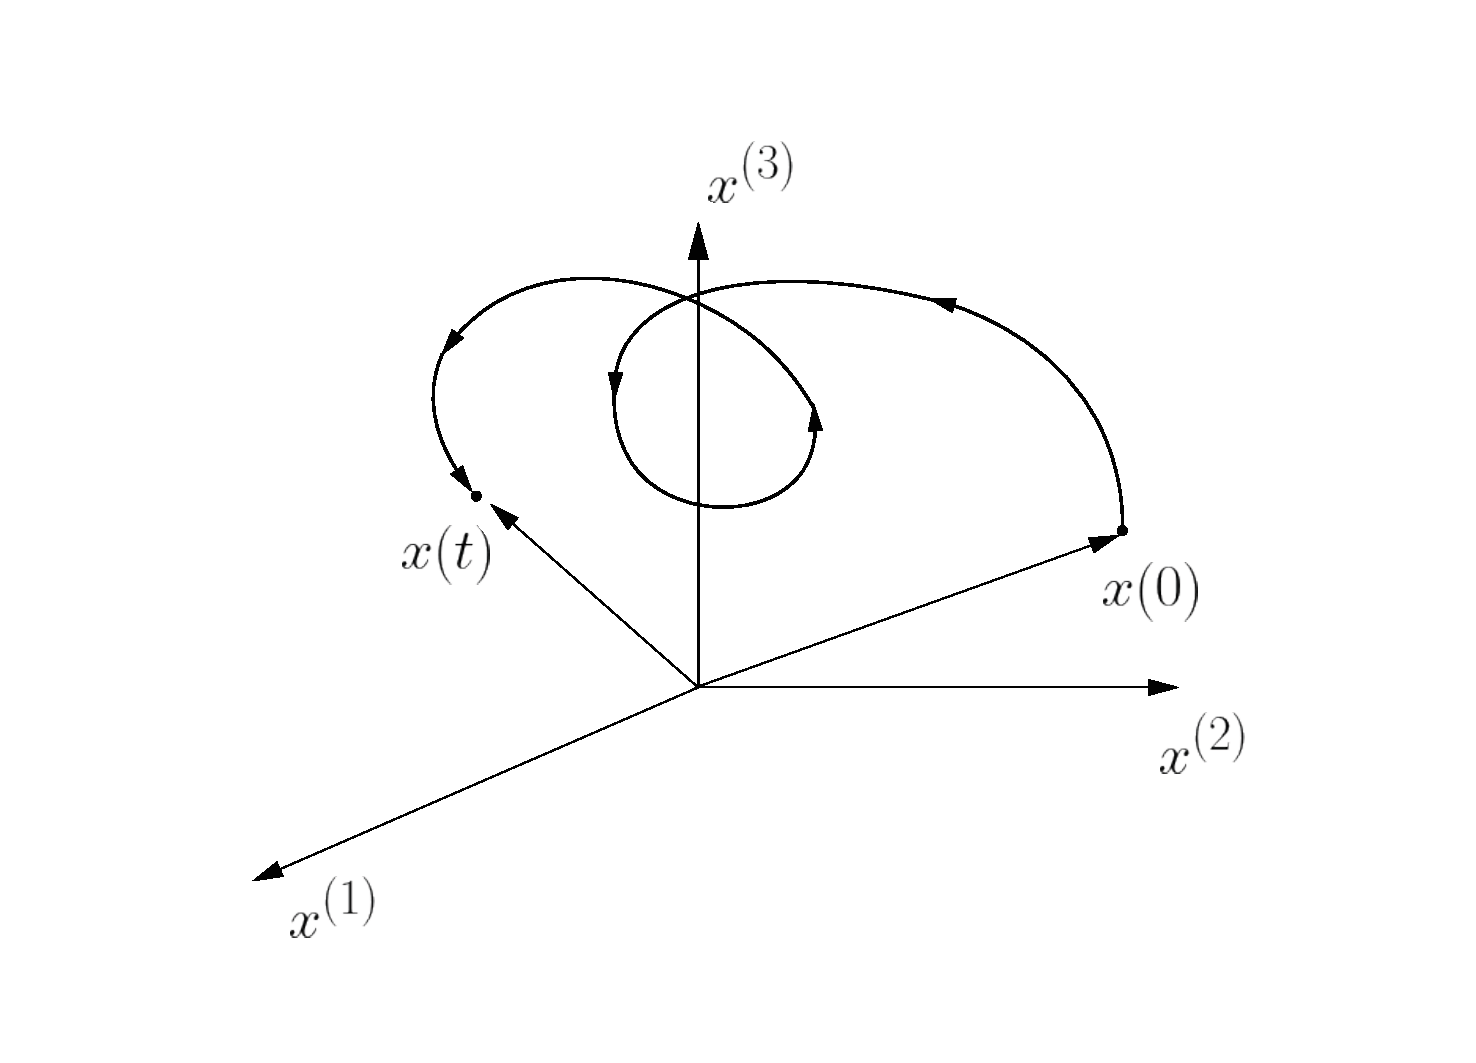
\includegraphics[width=1.\textwidth]{Figures/orbit_3d.pdf}
\caption{Orbit in three dimensional phase space}
\end{figure}

For the case of discrete systems, time is represented as integer values ($t=1,2,3,...$). An example of a dynamical system with discrete time is a map, which can be written as vector form as
\begin{equation}
\vec{x}_{t+1}=\vec{M}(\vec{x}_t)
\label{eq:discrete_dyn_sys}
\end{equation}
where $\vec{x}_t$ is an n-dimensional vector $\vec{x}_t=(x^{1}_t,x^{2}_t,...,x^{n}_t)$ and $\vec{M}$ a function of $\vec{x}_t$. Given an initial state $\vec{x}_0$, it is possible to obtain the state at time $t=1$ by $\vec{x}_{1}=\vec{M}(\vec{x}_0)$. Having determined $\vec{x}_1$ it will be possible to determine the state at time $t=2$ by $\vec{x}_2=\vec{M}(\vec{x}_1)$ and so on. Thus, given an initial condition $\vec{x}_0$ we generate a trajectory of the discrete time system: $\vec{x}_0,\vec{x}_1,\vec{x}_2,...$. 

A dynamical system that posses continuos time evolution may be reduced to a discrete time system by using the technique called Poincaré Surface Section. We consider a set of $n$ first order, autonomous, ordinary differential equations \ref{eq:set_diff_eqs}, a Poincaré map represents a reduction of the flow in the n-dimensional space to a map of dimension $n-1$. To illustrate this, an example with $n=3$ is given:

FIGURA\\
QUE\\
NO\\
HE\\
HECHO\\

Fig (NUMERO DE LA FIGURA) is a Poincaré section on a two dimensional plane $S$ on $x^{3}=constant$. The points A and B represent the succesive intersections of the trajectory followed by the system with the plane $S$, this crossing is always on the same direction. Given a point A, using Eq. (\ref{eq_:vect_diff_eqs}), we can determine the position of point B, this is because A can be used as an initial condition to determine B. The same argument can be used to determine A given B as initial condition by changing the sign of time on the same equation. Thus, the Poincar\'e map in this illustration represents an invertible two dimensional map transforming the coordinates $(x_n^{(1)},x_n^{(2)})$ of the $n$th piercing of the surface section to the coordinates $(x_{n+1}^{(1)},x_{n+1}^{(2)})$ at piercing $n+1$. This map can be generalized to an $N$ dimensional flow with an $N-1$ dimensional invertivle map.

\section{Hamilton equations and Symplectic Structure- OTT Y JOAO}

Hamiltonian systems are a class of dynamical systems that occur in a wide variety os circumstances. The special properties of Hamilton's equations endow these systems with attributes that differ qualitatively and fundamentally from other systems.\par 

The dynamics of a Hamiltonian system is completely specified by a single function, the Hamiltonian, $H(\bm{p},\bm{q},t)$. The state of the system is specified by its \say{momentum} and \say{position} usually known as $\bm{p}$ and $\bm{q}$ respectively, both vectors with dimension $N$. $N$ is also known as the number of degrees of freedom of the system. The Hamilton's equations determine the trajectory $(\bm{p}(t),\bm{q}(t))$ the system follows in the $2N$ dimensional phase space, these equations are given by

\begin{equation}
\frac{d \bm{p}}{dt} =-\frac{\partial H(\bm{p},\bm{q},t)}{\partial \bm{q}},
\label{eq:pdot_hamil}

\end{equation}
\begin{equation}
\frac{d \bm{q}}{dt} =\frac{\partial H(\bm{p},\bm{q},t)}{\partial \bm{p}}.
\label{eq:qdot_hamil}
\end{equation}
In the special case that the Hamiltonian has no explicit time dependance, $H=H(\bm{p},\bm{q})$, we can use Hamilton's equations to show that, as $\bm{p}$ and $\bm{q}$ vary with time, the value of $H(\bm{p}(t),\bm{q}(t))$ remains constant:
\begin{equation*}
\frac{dH}{dt}=\frac{d\bm{q}}{dt}\frac{\partial H(\bm{p},\bm{q})}{d\bm{q}}+\frac{d\bm{p}}{dt}\frac{\partial H(\bm{p},\bm{q})}{d\bm{p}}=\frac{\partial H(\bm{p},\bm{q})}{d\bm{p}}\frac{\partial H(\bm{p},\bm{q})}{d\bm{q}}-\frac{\partial H(\bm{p},\bm{q})}{d\bm{q}}\frac{\partial H(\bm{p},\bm{q})}{d\bm{p}}=0
\end{equation*}
Thus identifying the value of the Hamiltonian with the energy $E$ of the system, we see that the energy is conserved in the case of time independent systems, $E=H(\bm{p},\bm{q})=constant$\cite{ottChaosDynamicalSystems2002}.\par

Another particularity of Hamilton equations and Hamiltonian systems is that we can write Eqs. (\ref{eq:pdot_hamil},   \ref{eq:qdot_hamil}) in matrix form as
\begin{equation}
\frac{d\tilde{\bm{x}}}{dt}=\bm{F}(\tilde{\bm{x}},t),
\label{eq:symplectic1}
\end{equation}
by taking $\tilde{\bm{x}}$ to be the $2N$ dimensional vector
\begin{equation}
\tilde{\bm{x}}=\begin{pmatrix}
\bm{p}\\
\bm{q}
\end{pmatrix},
\end{equation}
and by taking $\bm{F}(\tilde{\bm{x}},t)$ to be 
\begin{equation}
\bm{F}(\tilde{\bm{x}},t)=\bm{S}_N \cdot \frac{\partial H}{\partial \tilde{\bm{x}}},
\label{eq:symplectic2}
\end{equation}
where $\bm{S}_N$ is the so called symplectic matrix given by 
\begin{equation}
\bm{S}_N=
\begin{bmatrix}
\bm{O}_N & -\bm{I}_N \\
\bm{I}_N & \bm{O}_N
\end{bmatrix}
\label{eq:symplectic_matrix}
\end{equation}
where $\bm{I}_N$ is the $N$ dimensional identity matrix, $\bm{O}_N$ is the $N \times N$ matrix of zeros, and
\begin{equation}
\frac{\partial H}{\partial \tilde{\bm{x}}}}=\begin{bmatrix}
\partial H / \partial \bm{p} \\
\partial H / \partial \bm{q}
\end{bmatrix}
\label{eq:sympl_hamil}
\end{equation}
From this we see how restricted the class of Hamiltonian systems is. In particular, a general system of the form (\ref{eq:symplectic1}) requires the specification of all the components of the vector function $\bm{F}(\tilde{\bm{x}},t)$, while by (\ref{eq:symplectic2}), if the system is Hamiltonian, it is specified by a single scalar function of $\bm{p}$, $\bm{q}$ and $t$ (the Hamiltonian).\par

One of the basic properties of Hamilton's equations is that they preserve $2N$ dimensional volumes in the phase space. This follows by taking the divergence of $\bm{F}(\tilde{\bm{x}})$ in Eq. (\ref{eq:symplectic1}), which gives
\begin{equation}
\nabla \cdot \bm{F}=\frac{\partial}{\partial \tilde{\bm{x}}}\cdot \bm{F}=\frac{\partial}{\partial \bm{p}}\Bigg(-\frac{\partial H}{\partial \bm{q}}\Bigg)+\frac{\partial}{\partial \bm{q}}\cdot \Bigg(\frac{\partial H}{\partial \bm{p}}\Bigg)=0
\end{equation}
Thus, if we consider an initial closed surface $S_0$ in the $2N$ dimensional phase space and evolve each point on the surface forward with time, we obtain at each instant	of time $t$ a new closed surface $S_t$ which contains within it precisely the same $2N$ dimensional volume as does $S_0$. This follows from

\begin{equation}
\frac{d}{dt}\int_{S_t}d^{2N}\tilde{\bm{x}}= \oint_{S_t}\frac{d\tilde{\bm{x}}}{dt}\cdot d\bm{S}=\oint_{S_t}\bm{F}\cdot d\bm{S}=\int_{S_t}\frac{\partial }{\partial \tilde{\bm{x}}}\cdot d^{2N}\tilde{\bm{x}}=0,
\end{equation}
where $\int_{S_t} \cdots$ denotes integration over the volume enclosed by $S_t$, $ \oint_{S_t}\cdots$ denotes a surface integral over the closed surface $S_t$, and the third equality is from the divergence theorem \cite{ottChaosDynamicalSystems2002}.. As a consequence of this result, Hamiltonian systems do not have attractors in the usual sense. This incompressibility of phase space volumes for Hamiltonian systems is called Liouville's theorem \cite{ottChaosDynamicalSystems2002}
CITAR AL GOLDSTEIN.\par

Perhaps the most important basic structural property og Hamilton's equations is that they are symplectic \cite{ottChaosDynamicalSystems2002}:
\begin{equation}
\frac{d\tilde{\bm{x}}}{dt}=\bm{S}_N\cdot \frac{\partial H}{\partial \tilde{\bm{x}}}.
\end{equation}
That is, if we consider three orbits that are infinitesimally displaced from each other, $(\bm{p}(t),\bm{q}(t))$, $(\bm{p}(t)+\delta \bm{p}(t),\bm{q}(t)+\delta \bm{q}(t))$ and $(\bm{p}(t)+\delta \bm{p}'(t),\bm{q}(t)+\delta \bm{q}'(t))$, where $\delta \bm{p}$, $\delta \bm{q}$, $\delta \bm{p}'$ and $\delta \bm{q}'$ are infinitesimal $N$ vectors, then the quantity,
\begin{equation}
\delta \bm{p}\cdot \delta \bm{q}'-\delta \bm{q}\cdot \delta \bm{p}',
\end{equation}
which we call the differential symplectic area, is independent of time,
\begin{equation}
\frac{d}{dt}(\delta\bm{p}\cdot\delta\bm{q}'-\delta\bm{q}\cdot\delta\bm{p}')=0.
\label{eq:sympl_area_no_time}
\end{equation}
The differential symplectic area can also be written as
\begin{equation}
\delta\bm{p}\cdot\delta\bm{q}'-\delta\bm{q}\cdot\delta\bm{p}'=\delta\tilde{\bm{x}}^{\dagger}\cdot\bm{S}_N\cdot \delta \tilde{\bm{x}}'
\label{eq:sympl_area_matrix}
\end{equation}
where $\dagger$ denotes transpose.\par

To derive (\ref{eq:sympl_area_no_time}) we differentiate (\ref{eq:sympl_area_matrix}) with respect to time and use Eqs. (\ref{eq:symplectic1}) - (\ref{eq:sympl_hamil}):

\begin{align}
\frac{d}{dt}(\delta \tilde{\bm{x}}^{\dagger}\cdot \bm{S}_N\cdot \delta \tilde{\bm{x}}')
&= \frac{d\delta \tilde{\bm{x}}^{\dagger}}{dt}\cdot \bm{S}_N\cdot \delta \tilde{\bm{x}}'+\delta \tilde{\bm{x}}^{\dagger}\cdot \bm{S}_N\cdot \frac{d\delta \tilde{\bm{x}}'}{dt}
\nonumber \\
&= \bigg(\frac{\partial \bm{F}}{\partial \tilde{\bm{x}}}\cdot \delta \tilde{\bm{x}}\bigg)^{\dagger}\cdot \bm{S}_N\cdot \delta \tilde{\bm{x}}'+\delta \tilde{\bm{x}}^{\dagger}\cdot \bm{S}_N \cdot \frac{\partial \bm{F}}{\partial \tilde{\bm{x}}}\cdot \delta \tilde{\bm{x}}'
 \nonumber \\
&= \delta \tilde{\bm{x}}^{\dagger}\cdot \Bigg[\bigg(\frac{\partial \bm{F}}{\partial \tilde{\bm{x}}}\bigg)^{\dagger}\cdot\bm{S}_N+\bm{S}_N\cdot \frac{\partial \bm{F}}{\partial \tilde{\bm{x}}}\Bigg]\cdot \delta\tilde{\bm{x}}'
\nonumber \\
&= \delta\tilde{\bm{x}}^{\dagger}\cdot\Bigg[\bigg(\bm{S}_N\cdot\frac{\partial^2 H}{\partial \tilde{\bm{x}} \partial \tilde{\bm{x}}}\bigg)^{\dagger}\cdot \bm{S}_N+\bm{S}_N\cdot\bm{S}_N\cdot\frac{\partial^2 H}{\partial\tilde{\bm{x}}\partial\tilde{\bm{x}}}\Bigg]\cdot\delta\tilde{\bm{x}}' \nonumber \\
&= \delta\tilde{\bm{x}}^{\dagger}\cdot\Bigg[\bigg(\frac{\partial^2 H}{\partial \tilde{\bm{x}} \partial \tilde{\bm{x}}}\bigg)^{\dagger}\cdot\bm{S}_N^{\dagger}\cdot \bm{S}_N+\bm{S}_N\cdot\bm{S}_N\cdot\frac{\partial^2 H}{\partial\tilde{\bm{x}}\partial\tilde{\bm{x}}}\Bigg]\cdot\delta\tilde{\bm{x}}' \nonumber \\
&=0,
\label{eq:proff_sympl_area}
\end{align} 
where we have used $\bm{S}_N\cdot\bm{S}_N=-\bm{I}_{2N}$ (where $\bm{I}_{2N}$ is the $2N$ dimensional identity matrix), $\bm{S}_N^{\dagger}=-\bm{S}_N$ and noted that $\partial^2H/\partial\tilde{\bm{x}}}\partial\tilde{\bm{x}}}$ is a symmetric matrix.Then the symplectic matrix $\bm{S}_N$ satisfies the folowing conditions CITE ARNOLD ERGODIC PROBLEMS OF CLASSICAL MECHANICS :
\begin{equation}
\bm{S}_N^{-1}=\bm{S}_N^{\dagger}=-\bm{S}_N
\end{equation}
and
\begin{equation}
det(\bm{S}_N)=1,
\end{equation}
which can be obtained directly form Eq.(\ref{eq:symplectic_matrix}).\par

Symplectic systems present a wide variety of properties CITE ARNOLD ERGODIC PROBLEMS OF CLASSICAL MECHANICS, but the one that is more relevant for this work, is that they conserve the volume on the $2N$ dimensional phase space, this means that symplectic dynamical systems follow the Liouville Theorem \cite{ottChaosDynamicalSystems2002}.\par

The fact that a Hamiltonian system conserves volume in the phase space has some consequences, we will highlight here the Poincar\´e  Recurrence Theorem CITE ZASLAVSKI HAMILTONIAN CHAOS AND FRACTIONAL DYNAMICS AND ZASLAVSKI THE PHYSICS OF CHAOS IN HAMILTONIAN SYSTEMS. When considering the movement of the system in a limited region of the phase space, which we denote as $Gamma$, wif we define a small area $A$ within this region (REF FIGURA QUE NO HE HECHO), with volume $\Gamma_A < \Gamma$, we can obtain a set of time values $\{ t_j\}$ for which the flow crosses this region from the inside out. The time intervals
\begin{equation}
\tau_j=t_{j+1}-t_j;\qquad j=0,1,2,...
\end{equation}
are the Poincar\´e Cycles and $t_j$ the Poincar\´e Recurrence Times. \par



FIGURA QUE NO HE HECHO DE LA REFERENCIA DE LOS CICLOS DE POINCARE\par

Poincar\´e proved that for a movement in a finite region of space in which the volume is preserved, the entire path sould return to a previously determined region (for example $A$ in Fig. FIGURA QUE NO HE HECHO) in a finite time and an infinite number of times. An exception occurs only if $A$ is a zero dimension set CITE ZASLAVSKI HAMILTONIAN CHAOS AND FRACTIONAL DYNAMICS AND ZASLAVSKI THE PHYSICS OF CHAOS IN HAMILTONIAN SYSTEMS.\par 

Thus, some general properties of Hamiltonian dynamical systems have been described. This ocurred without taking into account its movement, that is, its dynamics. In the coming sections, this question starts to gain space, focusing attention on some characteristics of its dynamics, more specifically when there is the presence of regular movement, chaos or a mixture of both.



\subsection{Integrability in Hamiltonian problems}
As we have previously stated, the case where the Hamiltonian has no explicit time dependence, $H=H(\bm{p},\bm{q})$, we have seen that Hamilton's equations imply that $dH/dt=0$ adn the energy $E=H(\bm{p},\bm{q})$ is a conserved quantity. Thus, orbits with a given energy $E$ are restricted to lie on the $(2N-1)$ dimensional surface $E=H(\bm{p},\bm{q})$. A function $f(\bm{p},\bm{q})$ is said to be a constant of motion of for a system with Hamiltonian $H$ is a constant of motion. More generally, differentiating $f(\bm{p},\bm{q})$ with respect to time, and assuming that there is no explicit time dependence of the Hamiltonian, we have
\begin{equation}
\frac{df}{dt}=\frac{d\bm{p}}{dt}\cdot\frac{\partial f}{\partial \bm{p}}+\frac{d\bm{q}}{dt}\cdot\frac{\partial f}{\partial \bm{q}}= \frac{\partial H}{\partial \bm{p}}\cdot\frac{\partial f}{\partial \bm{q}}-\frac{\partial H}{\partial \bm{q}}\cdot\frac{\partial f}{\partial \bm{p}}=0
\end{equation}
We call the expression appearing on the right hand side of the second equality the Poisson bracket of $f$ and $H$ CITAR AL GOLDSTEIN, and we abbreviate it as $\{F,h\}$. Using this definition, we have a condition for a function $f$ to be a constant of motion when the Hamiltonian does not depend on time CITE ZASLAVSKI HAMILTONIAN CHAOS AND FRACTIONAL DYNAMICS:
\begin{equation}
\{ f,H\} =0.
\end{equation}
(The Hamiltonian is a constant of the motion since $\{H,H\}=0$.)\par


For a system with $N$ degrees of freedom to be integrable, in the Liouville sence, it is necessary to exist $N$ constants independent of movement (or motion) $f_i(\bar{p},\bar{q})$(PIE DE PAGINA: If a constant cannot be described as a function of others, then it is called \say{independent} CITE OTT DYNAMICAL), with $i=1,2,...,N$ in such a way that
\begin{equation}
\{f_i,H\}=0
\label{eq:integrability_1}
\end{equation}
and 
\begin{equation}
\{f_i,f_j\}\delta_{ij}
\label{eq:integrability_2}
\end{equation}
where $\delta_{ij}$ is the kronecker delta, for all $i$ and $j$ CITAR HAMILTONIAN CHAOS AND FRACTIONAL DYNAMICS ZASLAVSKI. Said in another wat, the vectors $\bm{v_i}$, defined by
\begin{equation}
\bm{v_i}=\nabla f_i,
\label{eq:integrability_3}
\end{equation}
where $\nabla=(\partial/\partial q_1,...,\partial/\partial q_N,\partial/\partial p_1,...,\partial/\partial p_N)$ is the nabla operator of phase space, must be linearly independent at all the points in phase space CITE LIBRO DE MECANICA ANALITICA QUE DIGA ESO. If the conditions (\ref{eq:integrability_1})-(\ref{eq:integrability_3}) apply to any $i$ and $j$, then we say that the $N$ constants of motion are in involution.\par 

When an $N$ dimensional Hamiltonian system is integrable possesing $N$ independent constants of motion, the topology of the surface on which its trajectories evolve in the phase space are restricted to an $N$ dimensional torus CITE HAMILTONIAN CHAOS AND FRACTIONAL DYNAMICS ZASLAVSKI. For the case $N=2$, an orbit over a torus is shown in Figure (\ref{fig:trajectory_torus})

\begin{figure}[H]
\centering
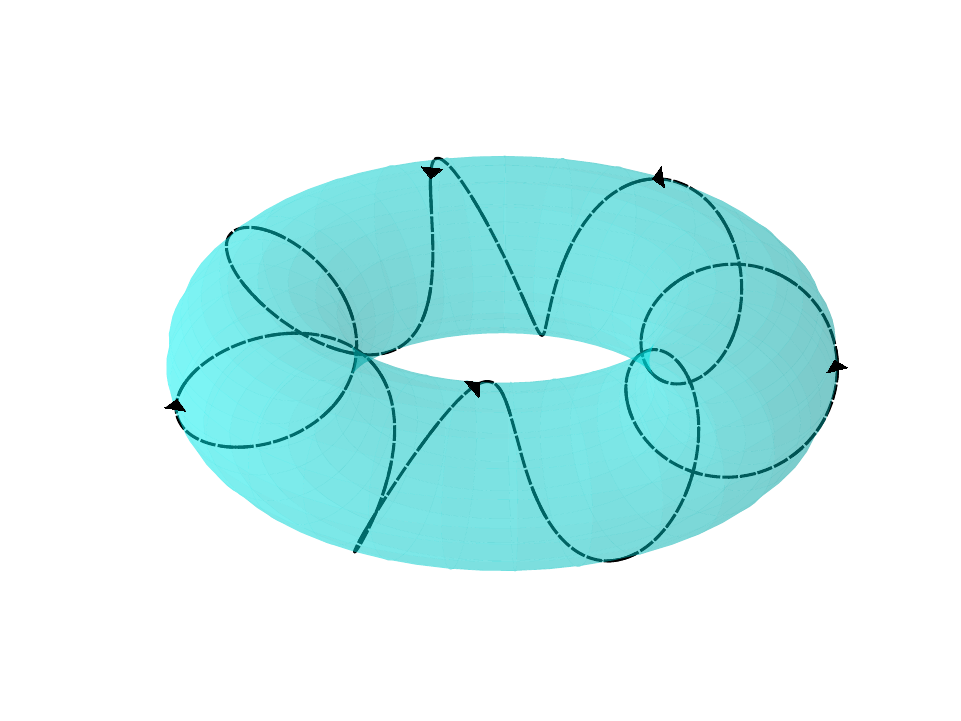
\includegraphics[width=0.7\textwidth]{Figures/trajectory_torus.png}
\caption{Trajectory on a torus for a bidimensional system with two constants of motion}
\label{fig:trajectory_torus}
\end{figure}

A simpler description of the movement of integrable Hamiltonian systems over the $N$ dimensional torus, can be made using the description in terms of the action-angle variables and the Hamilton-Jacobi equations, whose formalism can be found in Ref. CITAR AL GOLDSTEIN. For this, a canonical change of variables $(\bm{p},\bm{q})=\rightarrow (\tilde{\bm{p}},\tilde{\bm{q}})$ is introduced such that the Hamiltonian $\tilde{H}$ depends only on $\tilde{\bm{p}}$ and not on $\tilde{\bm{q}}$. This way, the Hamilton's equations with the new Hamiltonian become
\begin{equation}
\frac{d\tilde{\bm{p}}}{dt}= -\frac{\partial \tilde{H}}{\partial \tilde{\bm{q}}}=0  \qquad and \qquad  
\frac{d\tilde{\bm{q}}}{dt}= \frac{\partial \tilde{H}}{\partial \tilde{\bm{p}}}
\label{eq:action_angle_variables1}
\end{equation}
and $H(\bm{p},\bm{q})$ becomes $\tilde{H}(\tilde{\bm{p}})$.\par


Using the action-angle variables, we will write the components of the moment $\tilde{\bm{p}}$ and of the generalized coordinates $\tilde{\bm{q}}$ as
\begin{equation}
(\tilde{\bm{p}},\tilde{\bm{q}})=(\bm{I},\bm{\theta}),
\end{equation}
where the components of the action $\bm{I}_i$ are defined by CITAR AL GOLDSTEIN
\begin{equation}
\bm{I}_i=\frac{1}{2\pi}\oint p_idq_i \qquad where \qquad i=1,2,...,N.
\end{equation}
This way, we are writing the components of $\tilde{\bm{p}}$ as being $N$ constants of motion and at the same time satisfying Eq. (\ref{eq:action_angle_variables1}), since the time variation of a motion constant is zero.\par

In order to achieve the change of variables $(\bm{p},\bm{q})\rightarrow (\bm{I},\bm{\theta})$, we use the generating function $S(\bm{I},\bm{q})$ and the relations CITAR AL GOLDSTEIN
\begin{equation}
\bm{\theta}=\frac{\partial S(\bm{I},\bm{q})}{\partial \bm{I}} \qquad and\qquad \bm{p}=\frac{\partial S(\bm{I},\bm{q})}{\partial \bm{q}}
\end{equation}
because this function relates the \say{old} coordinates of the postion $\bm{q}$ and the \say{new} moment $\bm{I}$ CITAR AL GOLDSTEIN. With this, we can construct the Hamiltonian function in terms of the action-angle variables, $\tilde{H}(I)$ which is independent of $\theta$.\par

As said in the last paragraph, the new Hamiltonian is independent of $\bm{\theta}$ and the Hamilton equations Eq. (\ref{eq:action_angle_variables1}), can be written as 
\begin{equation}
\frac{d\bm{I}}{dt}=0 \qquad and \qquad \frac{d\bm{\theta}}{dt}=\frac{\partial \tilde{H}(\bm{I})}{\partal \bm{I}}\equiv \bm{\omega}(\bm{I}),
\label{eq:action_angle_variables2}
\end{equation}
their solutions are
\begin{equation}
\bm{I}(t)=\bm{I}(0)
\end{equation}
and
\begin{equation}
\bm{\theta}(t)=\bm{\theta}(0)+\bm{\omega}(\bm{I})t
\end{equation}
where each angle variable is periodic with a period of $2\pi$.\par

The second equation in Eq.(\ref{eq:action_angle_variables2}) can be interpreted as an angular velocity vector specifying trajectories over the $N$ dimensional torus CITAR AL GOLDSTEIN, where $\bm{I}$ represents the radius of the trajectory and $\bm{\theta}$ the angle of rotation. this fact is illustrated in Fig. FIGURA QUE NO HE HECHO DE LA SECCION TRANSVERSAL DEL TORO for the case where $N=2$. With the interpretation of $\bm{\omega}(\bm{I})$ as an angular velocity vector that specifies different paths over an $N$ dimensional torus, different types of movement over the torus can occur, which may be periodic or quasi-periodic, depending on the ratio between these frequencies. If there is an $N$ dimensional vector of integers $\bm{m}=(m_1,m_2,...,m_n)$, such that
\begin{equation}
\bm{m}\cdot \bm{\omega}=0,
\label{eq:rational_condition}
\end{equation}
except when $\bm{m}$ is a vector with all null components, the movement over the torus is a periodic movement and the ratio $\omega_1/\omega_i$ is a rational number. In these cases, the orbits followed by the system close on themselves after $m_1$ cycles cycles in $\theta_1$, $m_2$ cycles in $\theta_2$ and so on \cite{ottChaosDynamicalSystems2002}. When condition (\ref{eq:rational_condition}) is not satisfied and $\omega_1/\omega_i$ is an irrational number, the motion of the system is called quasi-periodic and an orbit never returns to its starting point, completely filling the surface of the torus \cite{ottChaosDynamicalSystems2002}.\par

When an integrable system begins to suffer the action of a disturbance, the tori whose ratio between frequencies is a rational or irrational number, behave in dfferent ways. The consequences of this disturbance on such tori  are explained by the KAM theorem, which we will describe later.


\subsection{KAM Theorem}
In the last subsections we introduced the necessary conditions for a system to be integrable. We also found that when the Hamiltonian is written in terms of the motion constants, especially in relation to the angle-action variables, the system's movement is limited to a rational or irrational $N$ dimensional torus, depending on the frequencies of the motion. But where does the integrability of a Hamiltonian system go? Or yet, what happens to rational and irrational tori when an integrable Hamiltonian system is subject to a disturbance? The answers to these questions came with the rigorous mathematical work of Kolmogorov, Arnold and Moser (KAM) and with the numerical studies developed on chaos and integrability after the advent of computer. The results obtained by Kolmogorov, Arnold and Moser became known as the KAM Theorem. The deduction of the theorem will not be detailed here, as it is ourside the scope of this work, only its results will be presented.\par

To describe the KAM theorem, we consider a disturbed Hamiltonian system, written in terms of the action-angle variables as
\begin{equation}
H(\bm{I},\bm{\theta})=H_0(\bm{I})+\epsilon H_1(\bm{I},\bm{\theta}),
\end{equation}
where $H_0(\bm{I})$ is the integrable Hamiltonian, $H_1(\bm{I},\bm{\theta})$ the perturbation and $(\bm{I},\bm{\theta})$ the action-angle variables of perturbed system.\par

The main idea of the KAM Theorem is to consider the effect of the disturbance on invariant Tori PIE DE PAGINA: A TORUS IS CALLED INVARIANT IF ONCE THE MOTION OF THE SYSTEM STARTS ON IT, THE MOTION STAYS ON IT. CITE OTT DYNAMICAL SYSTEMS. instead of the trajectories in the phase space CITE CHAOS AND FRACTIONAL DYNAMICS ZASDKJASD. In this way, we will divide the discussion into two cases, the Rational Torus and the Irrational Torus. We will se that many tori survive small disturbances, while others destroy themselves, giving rise to chaotic orbits, new tori and also elliptical and hyperbolic points.



\subsection{Rational Tori}
We call Rational Tori those whose ratio between the frequencies given by Eq.(\ref{eq:action_angle_variables2}) is a rational number. As a result of the action of the disturbance, these Tori are destroyed and it does not matter how small the values of $\epsilon$ are \cite{ottChaosDynamicalSystems2002}. Due to the destruction of the Rational Torus, there is the appeaance of an equal number of fixed elliptic and hyperbolic points. This result is known as the Poincar\´e Birkhoff theorem CITE REGULAR AND CHAOTIC DYNAMICS LICHTENBERG LIEBERMAN . The number of fixed points that appear depends on the ratio between the frequencies of the rational torus. If we call $R=\tilde{p}/\tilde{q}$ the torus rotation number, where $\tilde{q}$ represents the largest number of cycles performed on the torus before the path returns over itself, then, due to the disturbance, there will appear an equal or multiple number of $\tilde{q}$ of elliptical points and hyperbolic points \cite{ottChaosDynamicalSystems2002}. Fig. (FIGURA QUE NO HE HECHO DEL TORO RACIONAL PERTURBADO POCAMENTE) illustrates a case where $\tilde{q}=3$ and $\tilde{q}=4$ in a Poincar\´e section for a system with $N=2$.\par

These elliptical and hyperbolic points that result from the breakdown of the rational torus due to the perturbation, they remain fixed points of the disturbed system and with the same perio $\tilde{q}$ of the rational torus CITE REGULAR AND HAOTIC DYNAMICS LICHTENBERG LIEBERMAN . The difference between the two points is in the way initial conditions close to them behave. Next to fixed elliptical points, new curves appear similar to those that existed before the perturbation, which we call KAM curves, some of which are rational and others irrational. Such fact is presented inside the box on Fig. (FIGURA ANTERIOR LA PARTE B TIENE UNA CAJA CERRADA DE UN PUNTO ELIPTICO). When these rational KAM curves that appeared due to the action of the disturbance are destroyed, other elliptical and hyperbolic points will appear, surrounded again by rational and irrational KAM curves and so on \cite{ottChaosDynamicalSystems2002}.\par

Orbits enerated near hyperbolic points, can have different behaviors, because hyperbolic points, also known as saddle points, have stable directions or varieties, those that move to the fixed point, or unstable, those who move away from it \cite{ottChaosDynamicalSystems2002}. If we follow the varieties, moving away from a fixed point, they will usually present homoclonic or heteroclonic intersections, which occur when unstable varieties from the same point cross over themselves or from two different points intersect at different points, respectively \cite{ottChaosDynamicalSystems2002}. Fig. (REF FIGURA QUE NO HE HECHO DE LOS ENREDAMIENTOS HOMOCLINICOS) represents these crossings for a single point and for two distinct hyperbolic points.\par 

Thus, the destruction of the rational torus not only generates stable elliptical points, but also generates hyperbolic points, which are responsible for the chaotic movement, which is always trapped by the KAM curves that haven't been \say{broken} \cite{ottChaosDynamicalSystems2002}, at least for an $N=2$ case. As these curves begin to \say{break}, more and more chaotic regions are appearing, completely filling with points the allowed region of the Poincar\´e section. We will now see what is the sequence in which the irrational torus gives rise to the elliptical and hyperbolic points.
FIGURA\par
QUE\par
NO\par
HE\par
HECHO\par
DE\par
LOS\par
PUNTOS\par
Y\par
CRUZAMIENTO\par
HOMOCLINICO\par





\subsection{Irrational Tori}
When an integrable system is disturbed, the KAM Theorem guarantess the existence of a torus in the phase space, if te conditions below are met:
\begin{enumerate}
\item The torus' linear frequencies of the integrable system are independent	 CITE REGULAR AND CHAOTIC DYNAMICS LICHTENBERG LIEBERAN, that is, we hae a torus whose ratio between the frequencies is an irrational number.
\item The perturbation is a smooth function CITE REGULAR AND CHAOTIC DYNAMICS LICHTENBERG LIEBERAN (a sufficient number of derivaties of $H_1$).
\item Initial conditions are sufficiently far from the rational tori CITE REGULAR AND CHAOTIC DYNAMICS LICHTENBERG LIEBERAN.
\end{enumerate}
With the above conditions satisfied, the KAM Theorem guarantess the existence of deformed torus, with the same topology as the unperturbed torus, in the vicinity of te irrational torus of the system in the non-perturbed. These tori that appear deformed after the perturbation are called the KAM Tori.\par

The that the irrational torus must be sufficiently far from the rational torus, for the existence of the KAM Tori, implies that the more irrational the ratio between the frequencies of the non-perturbed tori, the easier it is for the KAM Tori to appear CITE REGULAR AND CHAOTIC DYNAMICS LICHTENBERG LIEBERAN.\par

The idea of more irrational numbers can come with the help of number theory. An irrational number $R$ can  be represented as an infinite continuous function \cite{ottChaosDynamicalSystems2002}:
\begin{equation}
R=a_1+\frac{1}{a_2+\frac{1}{a_3+\frac{1}{a_3+ \cdots}}}
\end{equation}
where the $a_i$'s are integer numbers. However, if the integers $a_i$'s for $i\geq k$ are equal to one, this irrational number is called \say{noble} CITE ORDER AND CHAOS IN DYNAMICAL ASTRONOMY CONTOPOULOS. The \say{most irrational} numer that exists is consequently the most \say{noble} of them all CITE ORDER AND CHAOS IN DYNAMICAL ASTRONOMY CONTOPOULOS, and it is the golden ratio
\begin{equation}
R=\frac{(\sqrt{5}-1}{2}
\end{equation}
When the most \say{noble} number of all is related to the irrationality of a KAM Tori, it will be the last one to be destroyed as the intensity of the perturbation is increased. However, if it is not present, the last KAM Tori to be destroyed will be the one with the most \say{noble} number CITE ORDER AND CHAOS IN DYNAMICAL ASTRONOMY CONTOPOULOS.\par

In general, the effect of the perturbation on an integrable system can be summarized as follows: When the disturbance begins to act on the integrable system, many tori of the integrable system are slightly deformed and survive (Irrational Tori), while others are destroyed (Rational Tori). Regions close to the tori that were not destroyed by the perturbation are occupied by new irrational orbits, elliptical points, hyperbolic orbits and chaotic orbits. As the disturbance increases, the irrational tori destroy themselves, the last one to be \say{destroyed}, is the one that has the value of the ratio between the frequencies as a \say{more noble} number.\par

When the perturbation on the integrable system breaks all tori, including the \say{noblest}, the system starts to present characteristics such as ergodicity, drops of correlations, etc...



\section{Symplectic Integrator NUMERICAL HAMILTONIAN PROBLEMS}
As we said previously, symplecticness is a very important property of the Hamiltonian. Numerical integrators are generally speaking numerical mappings of the differential equations, generally these mappings are nonsymplectic. Applying nonsymplectic algorithms to hamiltonian problems tend to show solutions where the area in phase space is not conserved as is showed below


\begin{figure}[H]%
    \centering
    \subfloat[Position dynamics]{{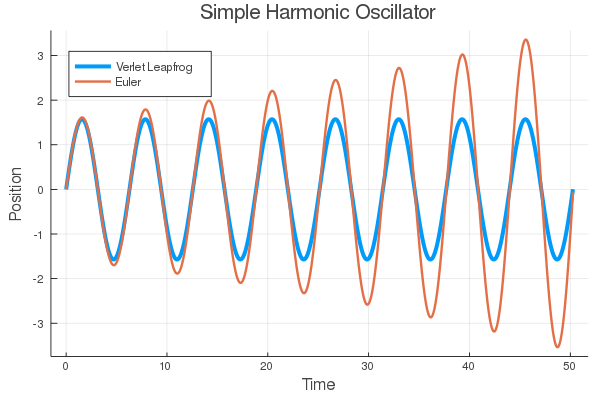
\includegraphics[width=10cm]{Figures/harmonic_oscillator.png} }}%
    \qquad
    \subfloat[Phase space dynamics]{{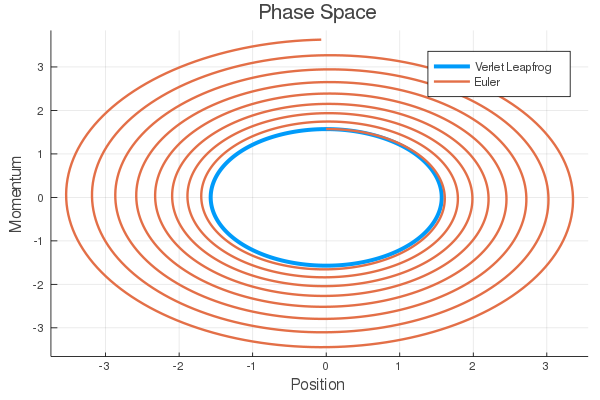
\includegraphics[width=10cm]{Figures/harmonic_oscillator_PS.png} }}%
    \caption{Euler non symplectic integrator compared to symplectic Verlet Leapfrog method}}%
    \label{fig:euler}%
\end{figure}

This failure of mimicking well known Hamiltonian dynamics suggested the consideration of schemes that generate a symplectic mapping $Psi$ when applied to Hamiltonian problems. Such methods are called symplectic or canonical. Early references on symplectic integration are CITAR A RUTH CHANNEL MENYUK FENG, even though the idea of symplectic integration apparently goes back to DeVogelaere in 1956 CITAR CHANNEL SCOVEL 1990.

\subsection{Importance of symplecticness in an integrator}
A symplectic integrator is then an integrator whose solution resides on a symplectic manifold. Because of discretization error, when it is solving a Hamiltonian system it doesn't get exactly the correct trajectoy on the manifold. Instead, that trajectory itself is perturbed $\mathcal{O}(\Delta h^n)$ for the order $n$ from the true trajectory. Then there's a linear drift due to numerical error of this trajectory over time. Normal integrators tend to have a quadratic (or more) drift, and do not have any good global guarantees about this phase space path, it only guarantees the path in a local sense.\par




What this tends to mean is that symplectic integrators tend to capture the long-time patterns better than normal integrators because of this lack of drift and this almost guarantee the periodicity of certain problems. 

\subsection{Conservation of constants of motion}
As we have seen previously, when one uses a symplectic integrator of order $n$ what you do is to solve in an exact way the evolution of the system, but not using the hamiltonian $H$ but one softly perturbated as $\tilde{H}=H+\epsilon H_1$, where $\epsilon=t^n$ and $H_1=H_1^0+hH_1^1+h^2H_1^2+...$ If what we really want to obtain is a qualitative information of the behavior of the system, we can expect that if $\epsilon H_1$ is sufficiently small, the system will evolve in a very similar way for $\tilde{H}$ as for $H$.\par

Consider now a system that has $m$ independent constants of motion $J_i$ where $i=1,...,m$, this means that for every $J_i$ it satisfies the condition of a null poisson bracket with the hamiltonian as $\{H,J_i\}=0$. As the integrator is solving in an exact way the evolution due to the hamiltonian $\tilde{H}$, it will follow that the constants of motion, in general, will not be constant as they will not have a null poisson bracket, in principle, with this new hamiltonian. Nonetheless, the following is obtained
\begin{equation}
\{\tilde{H},J_i\}=\{H+\mathcal{O}(h^n),J_i\}=\mathcal{O}(h^n).
\end{equation}
Despite some exceptions, the constants of motion $J_i$ will not be constant along the evolution of the system, but they will disagree to being it in the same order as the energy does. Therefore, for an efficient integrator with high order precision the constants of motion will certainly be constant along the dynamical trajectory.




\subsection{Chaos and integrators TOCA METERLE VARIAS REFERENCIAS}

Numerical chaos has been a very interactive branch of study for many years since the surge of computers. As we have shown, numerical stability of differential equations is very sensitive to systems involving chaos, even the slightest difference on the floating point error gives rise to diverging trajectories in phase space, this makes chaotic systems very interesting problems numerically speaking. As we know, floating numbers that computer algorithms work with have a finite value for decimals, when coputing a solution of a differential equation using a given algorithm computers truncate this decimals leaving some round-off error. These truncations are not overseen by chaotic systems, chaotic systems has the nature to amplify the slightest perturbance of the system into an observable result, this means that numerical truncations on floating point numbers have long term consequences when interpreting what we consider the solution. It is necessary to take into account these considerations when solving a chaotic system.\par

Numerical integrators and chaos consequently gather on an exotic dance of conditions to consider, on one hand it is important for integrators to have a high order of accuracy by using intermediate steps before computing a definitive step on the trajectory of the solution and it is also important to have a small enough integration step to manage sensibility for the trajectory; on the other hand, error propagation of the floating point decimal truncation everytime the integrator performs an operation discourages all the effort put into calculating derivatives using intermediate steps and raises the question on what is the important aspect to consider. The answer is often unknown, solving these numerical problems with optimal efficiency is truly a very complicated task for the majority of chaotic problems.



\section{Randomness in classical and quantum mechanics}

Randomness and chaos share similarities physically speaking, they amplify any type of noise from the microscopical degrees of freedom and show them visible in the outcome of the dynamics of the systems. The idea to achieve true randomness on experiments or random number generators is a dream for many experimentalists, but the true situation is that most of the times, classically you can't have the perfect un-biased scenario of randomness. One great example is illustrated bu Diaconis et al. CITAR PAPER DIACONIS MONEDA where very precise measurements and theroretical descriptions are applied to the commonly known random event of the coin toss. The outcome of this research is that for natural flips the result of the coin is biased to come up as started $51%$ of the times. Another example of a physical method to come up with random numbers is related to optical chaos CITAR A (Li, Pu; Wang, Yun-Cai; Zhang, Jian-Zhong (2010-09-13). "All-optical fast random number generator". Optics Express. 18 (19): 20360–20369. Bibcode:2010OExpr..1820360L. doi:10.1364/OE.18.020360. ISSN 1094-4087. PMID 20940928.
Li, Pu; Sun, Yuanyuan; Liu, Xianglian; Yi, Xiaogang; Zhang, Jianguo; Guo, Xiaomin; Guo, Yanqiang; Wang, Yuncai (2016-07-15). "Fully photonics-based physical random bit generator". Optics Letters. 41 (14): 3347–3350. Bibcode:2016OptL...41.3347L. doi:10.1364/OL.41.003347. ISSN 1539-4794. PMID 27420532.
), it has  has a high potential to physically produce high-speed random numbers due to its high bandwidth and large amplitude. A prototype of a high speed, real-time physical random bit generator based on a chaotic laser was built in 2013 CITAR A (Wang, Anbang; Li, Pu; Zhang, Jianguo; Zhang, Jianzhong; Li, Lei; Wang, Yuncai (2013-08-26). "4.5 Gbps high-speed real-time physical random bit generator". Optics Express. 21 (17): 20452–20462.).\par


Determinism defined as the property of events to be determined completely by previously existing causes is an important concept concerning classical mechanics, given the equations of motion of a system, we know in an exact way the state of the system in a future time with arbitrary precision. Chaotic systems are very sensitive to small changes on the initial conditions and they are often missunderstood as random, but as we have previously described, chaotic systems do not exhibit random behavior in the sense that it can be at any place located in phase space but we have shown that it certainly remains conditioned by a certain degree to the motion on the KAM tori giving place to quasiperiodicity.\par 

On the other hand, quantum mechanics seems to have fundamental randomness in its roots, measurements are regarded as probability measurements of the system to be in a determined state.  The Born's interpretation of the quantum mechanics of the wave function implies that we can count only on a probabilistic description of reality, therefore quantum mechanics is inherently probabilistic CITAR LA INTERPRETACION DE BORN DE QM. Randomness in quantum mechanics is also regarded to be due to the interaction of a measurement apparatus and an environment with the initial pure states. This is consistent and parallel to the modern way of intepretations of the collapse of the wave functions and the quantum measurements CITAR A WHEELER AND ZUREK 1983 ZUREK 2003 Y ZUREK 2009.\par 

It is important for us to talk about the experiment to measure a spin component along a direction. If we take the $z$ component  as an example similar to the Stern-Gerlach experiment CITAR EL EXPERIMENTO DE STERN GERLACH, in this experiment the particles before the measurement are regarded to be in a neutral state along the $z$ component, after the particles go through the inhomogeneous magnetic field the spin aligns along a direction of the $z$ component and gets deflected along this direction. The result of the experiment is seen in a screen where two clouds of particles are seen, one in the upper location and one in the lower one. The counts of particles on each cloud is the same in both cases, this translates as the probability of the particles to be aligned along certain direction is the same. Particles then have a completely random probability to the aligned along certain direction, this idea can be compared with the one of the coin toss, only two possible outcomes of the measurement. There is a big difference between both pictures besides one being classical and the other one quantum, it is that the coin toss is not truly random as it depends strongly on the initial conditions on how the coin toss is made meanwhile the spin measurement seems to be totally random as long as the particle is initially in a non-commuting state with the $z$ component of the spin. This idea is the one we are going to exploit on the next chapters and explore a little bit the grounds of the environment and its role of introducing bias to the outcome of the measurements.


